\documentclass[conference]{IEEEtran}
\IEEEoverridecommandlockouts
\usepackage{cite}
\usepackage{amsmath,amssymb,amsfonts}
\usepackage{algorithmic}
\usepackage{graphicx}
\usepackage{textcomp}
\usepackage{xcolor}
\usepackage{multirow}
\def\BibTeX{{\rm B\kern-.05em{\sc i\kern-.025em b}\kern-.08em
    T\kern-.1667em\lower.7ex\hbox{E}\kern-.125emX}}
\begin{document}

\title{Smart Spreading Factor Assignment for LoRaWANs}


\author{\IEEEauthorblockN{Tugrul Yatagan and Sema F. Oktug}
\IEEEauthorblockA{Department of Computer Engineering,
Istanbul Technical University\\
Istanbul, Turkey\\
Email: \{yatagan, oktug\}@itu.edu.tr}}
\maketitle


\begin{abstract}
Low power wide area network (LPWAN) technologies offer affordable connectivity to massive number of low-power devices distributed over very large geographical areas. Focus of this work is one of the most promising LPWAN technologies: LoRa. LoRa offers long range communication and strong resilience to interference by proprietary modulation technique based on Chirp Spread Spectrum (CSS). LoRa modulation trades data rate for sensitivity and communication range by spreading symbols within a fixed channel bandwidth. Collisions in LoRaWAN networks are strongly related with spreading factor (SF) assignment of nodes which indeed effects network performance. In this work, a simulation environment to study different SF assignment schemes is implemented. Furthermore, a novel SF assignment strategy is proposed which utilizes a machine learning technique for optimization of SF assignment. Finally, promising simulation results for proposed machine learning SF assignment technique is presented.
\end{abstract}


\begin{IEEEkeywords}
LoRa, Spreading Factor, IoT, LPWAN, Machine Learning
\end{IEEEkeywords}


\section{Introduction}
\par In the last few years, number of Internet of Things (IoT) applications increased exponentially \cite{7721743}. Recent developments on LPWAN technologies has great impact on growth of number of IoT applications. LPWAN technologies address some of the well-known wireless communication challenges. Traditional wireless communication methods such as cellular networks (e.g., 2G, 3G, LTE) and short-range communication technologies (e.g., Bluetooth, WiFi, Zigbee) cannot provide low power and long range at the same time. Cellular networks can provide long range and high data rate, but they are complex and consume too much power. Besides, most of the IoT applications do not require high data rate. Short-range communication methods can provide relatively low power consumption, but their range is limited to a few hundred meters at best \cite{7815384}. LPWAN technologies fill the technology gap between short range and cellular technologies by providing low power and long-range communication. LPWAN technologies basically sacrifice data rate to provide low power consumption.

\par There are several emerging LPWAN technologies. LoRa, Sigfox, NB-IoT and LTE-M are commonly used, well-known LPWAN technologies. LoRa and Sigfox use license free ISM frequency bands while NB-IoT and LTE-M use licensed frequency bands which brings extra cost \cite{7815384}. Both LoRa and Sigfox are known for ultra-low power consumption and resilience to interference. While NB-IoT and LTE-M are promoted for higher data rate. LoRa has open standard MAC protocol called LoRaWAN. LoRaWAN and Sigfox MAC protocols are based on pure ALOHA medium access. LoRaWAN networks can be deployed as a private network like WiFi. However, Sigfox and NB-IoT are only available with operator contract \cite{7815384}.

\par LoRa can adjust data rate by spreading symbols within a fixed channel bandwidth. This enables tradeoff between receive sensitivity and transmission time on air \cite{7803607}. Simultaneous same spreading factor (SF) transmissions are prone to collision, however, different SF transmissions in the same channel are orthogonal to each other, thus SF assignment is crucial for overall network performance. In this work, a LoRa discrete event simulator is developed to study different LoRa SF assignment strategies. We also proposed an SF assignment scheme to increase network performance with the help of machine learning methods and we verified our proposal using the simulator.

\par The following two sections provides a background information about LoRa and LoRaWAN. Section \ref{Other Related Works} describes other related works. Section \ref{Proposed Technique} describes proposed technique for SF assignment. Simulation environments and results are shown in Section \ref{Simulation Environment} and \ref{Simulation Results}. Finally, Section \ref{Conclusion} concludes the paper.


\section{LoRa}
\par LoRa is the name of the proprietary physical layer radio/chipset technology that provides wireless link solution for low power wide area networks. LoRa is designed and patented by Semtech Corporation. LoRa uses proprietary spread spectrum modulation technique that is derivative of Chirp Spread Spectrum (CSS). A chirp is a sinusoidal signal which its frequency increases over time. Chirp frequency increases linearly and sweeps the entire bandwidth. We invite readers to refer to \cite{AN1200.22} for further details.

\subsection{Spreading Factor}
\par Spreading factor (SF) is the ratio between symbol rate and chirp rate. The ratio between symbol and chirp rate is equal to $2$\textsuperscript{SF}. SF can take values between 7 to 12. SF also determines data rate of a LoRa transmission \cite{AN1200.22}. Data rate of a LoRa transmission can be calculated as:

\begin{equation} \label{eq:bit_rate_sf}
R_{b} = SF * \dfrac{\left[ \dfrac{4}{4+CR} \right] }{ \left[ \dfrac{2^{SF}}{BW|_{Hz}} \right]} \ bps
\end{equation}

Where, $R_{b}$ is data rate in bps, SF is spreading factor $SF \in \{7,..,12\}$, CR is error correction code rate $CR \in \{1,..,4\}$ and $BW$ is bandwidth in Hertz \cite{AN1200.22}.

\par When BW and CR are constant, as the SF increases, the data rate decreases. Increasing the SF makes the signal more resilient to noise thus increases the transmission range. Increasing the SF also increases the transmission duration which increases the power consumption. Therefore, it is possible to trade between range and power consumption by changing SF.

\subsection{Spreading Factor Assignment Issue}
\par Simultaneous different SF transmissions are orthogonal to each other up to some extent. Which means, a LoRa gateway can simultaneously receive multiple transmissions with different SFs. However, simultaneous transmissions with same SF may not be received by gateway due to collision. For this reason, spreading factor assignment of nodes is crucial for network performance.

\par In a LoRaWAN network, initially, a node is not aware of how far it is from a GW. However, a node can guess the distance from a gateway by observing received signal power of a downlink transmission. If a downlink transmission received signal power is too high, then node can decrease its next transmission SF to decrease power consumption. This SF assignment method is called lowest possible SF assignment scheme for the rest of the paper. Also, a GW can request from a node to decrease node's SF or transmit power.

\par In Figure \ref{fig:collision}, a LoRaWAN network deployed with a single GW is illustrated. Different color rings represent achievable range of different SFs from the GW and different color circles represent selected SF of the nodes. Most of the end devices which close to the GW will fall into lowest SF (SF7) area section. End devices which close to the GW will probably select lowest SF all the time. This results a lot of collisions between same SF transmissions. Number of collisions increases while number of end devices close to the GW increases.

\begin{figure}
\centering
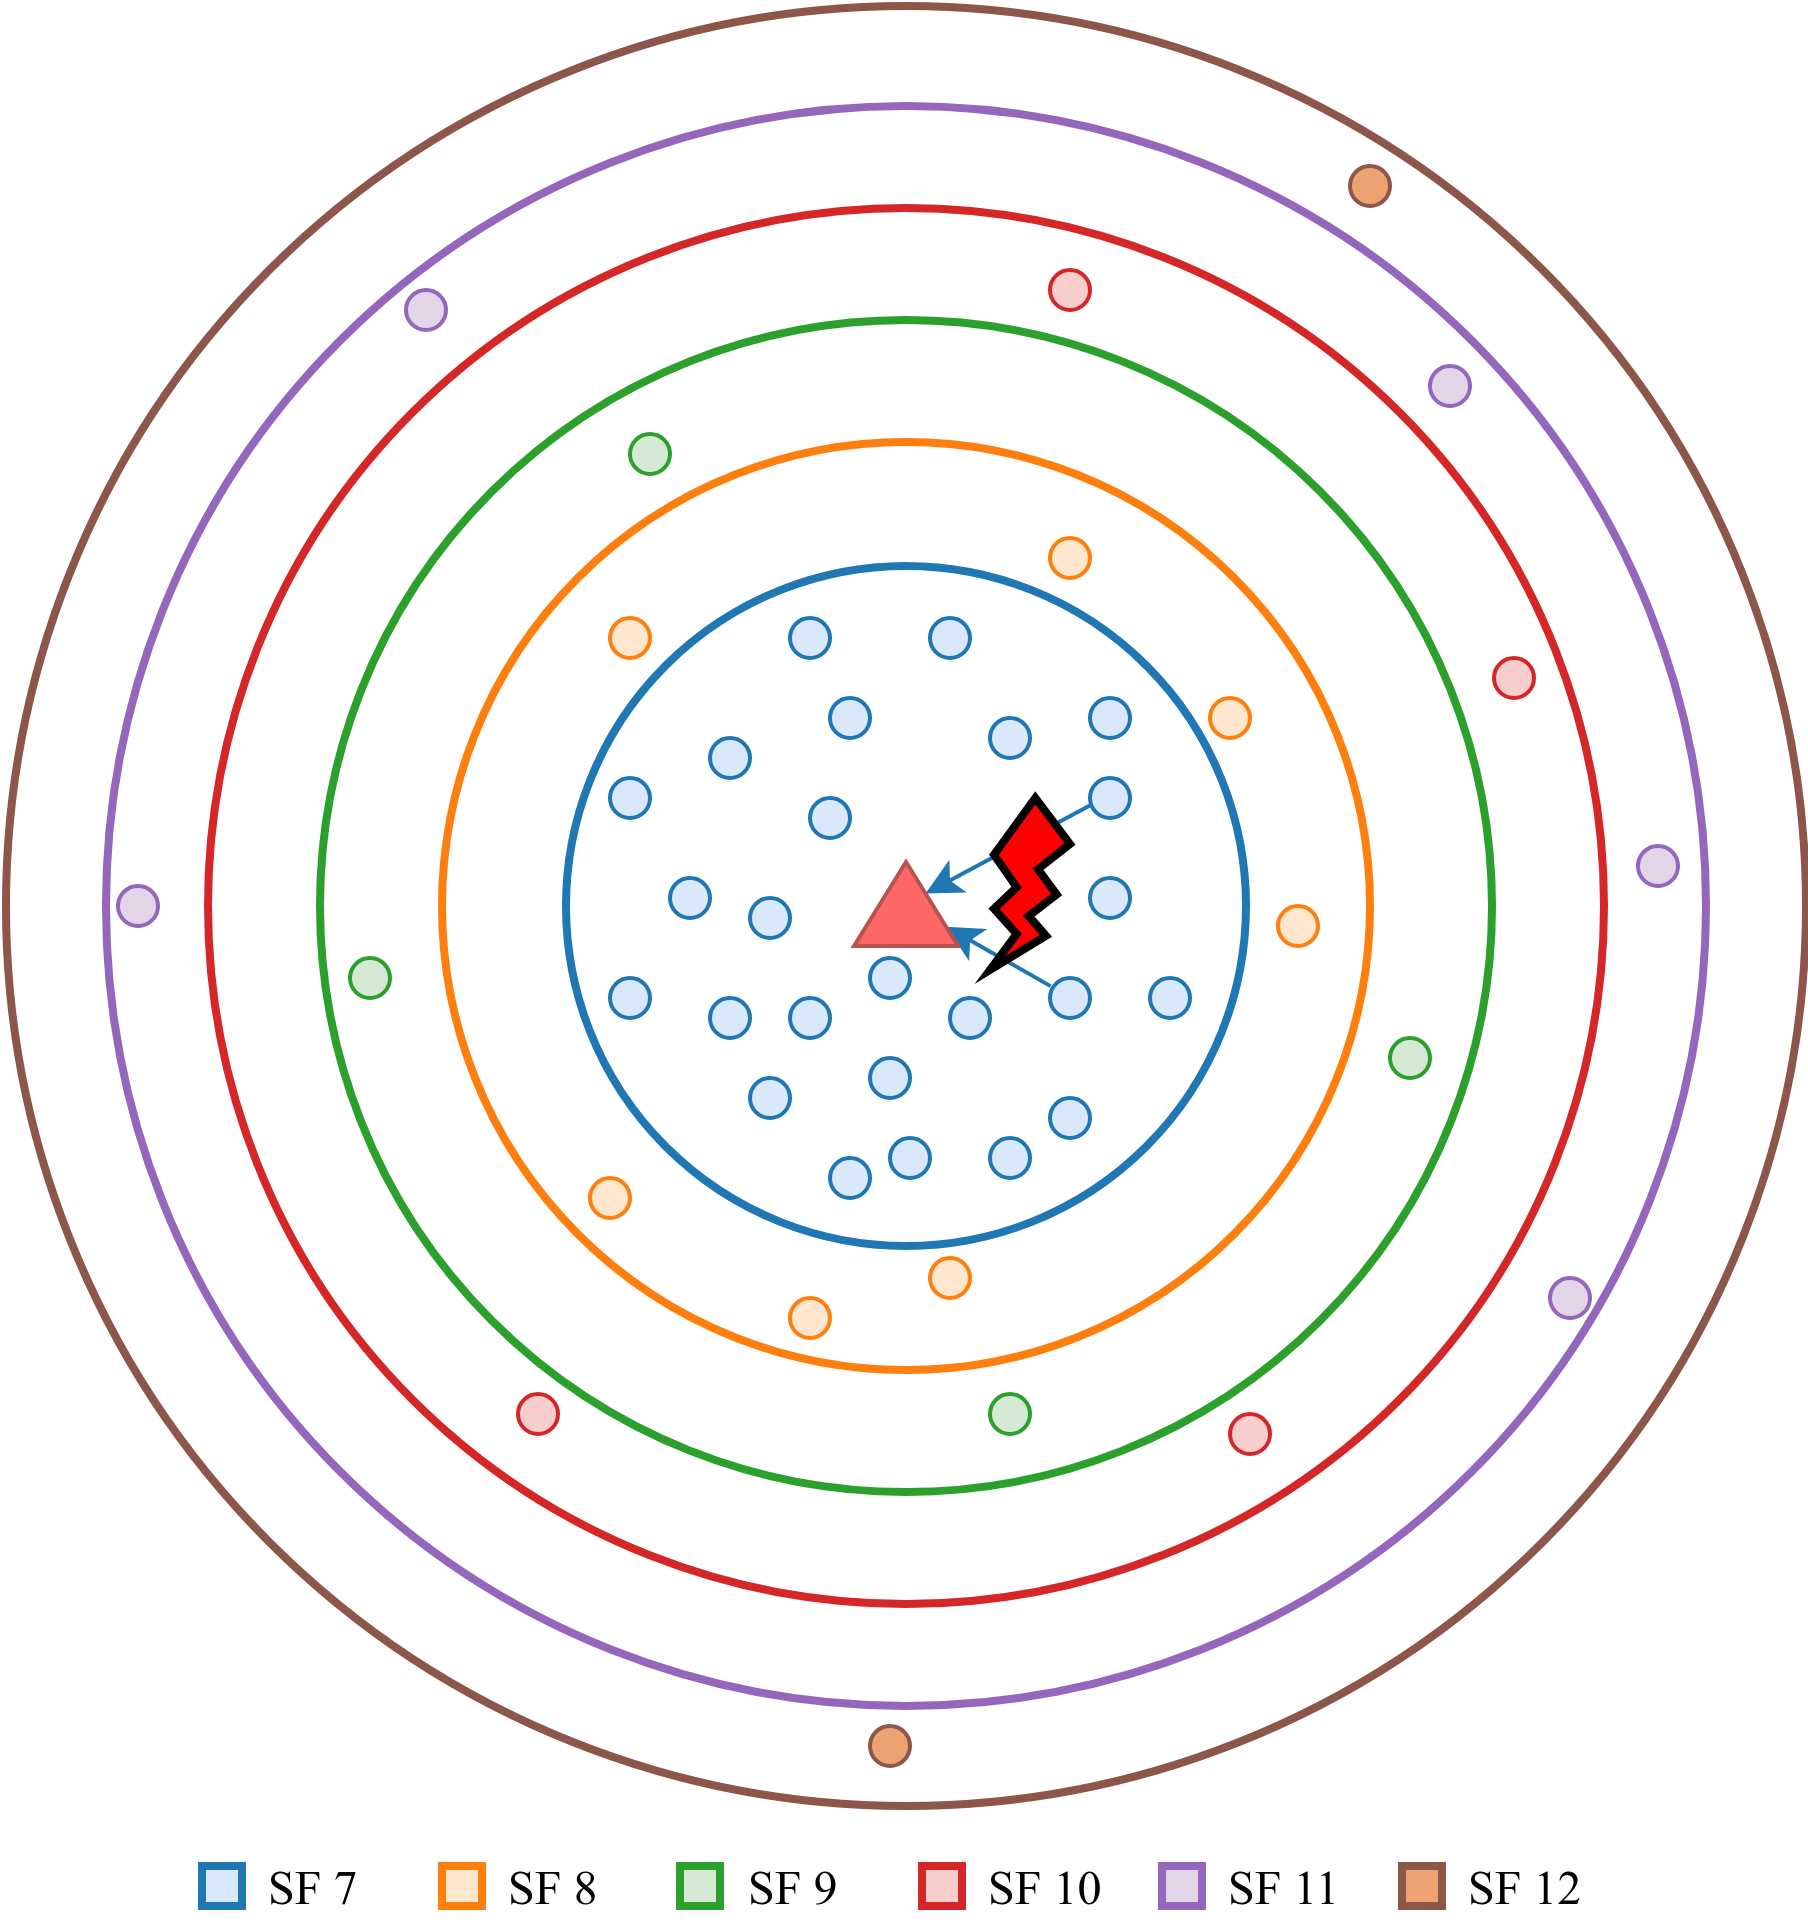
\includegraphics[width=\linewidth]{collision}
\caption{Collision between nodes close to the GW.}
\label{fig:collision}
\end{figure}


\section{LoRaWAN} \label{LoRaWAN}
\par LoRa has an open standard medium access control (MAC) layer protocol called LoRaWAN. LoRaWAN is a medium access control (MAC) layer protocol which designed for large scale LoRa networks. LoRaWAN is developed and maintained by LoRa Alliance. LoRa Alliance is an open, non-profit organization dedicated to standardization of LoRaWAN. LoRaWAN  provides inter-operability between different LoRa networks. LoRaWAN is based on pure ALOHA medium access which means end nodes do not check whether the channel is free or not before transmitting, accepting the possibility of the collision.

\par A typical LoRaWAN network consist of three network entities.

\subsection{End node}
\par LoRaWAN end node (EN) is a low power embedded device that only communicates to gateways. LoRaWAN standard defines three classes for end devices which are Class A, Class B, and Class C. Different classes provides LPWAN solutions to different deployments and topologies. Class A end nodes generate uplink transmission at any time and only receives a period of time after uplink transmission. Class B end nodes extend Class A behavior by adding scheduled receive windows for downlink transmission. Receive window is synchronized using a beacon packet transmitted by gateways. Class C end nodes extend Class A behavior by keeping receive window open all the time except uplink transmission. This provides Class C end nodes to low latency downlink communication, but it requires more power consumption. In this paper, we focused on Class A end devices since Class A behavior provides the lowest power consumption.

\subsection{Gateway}
\par LoRaWAN gateway (GW) is a device that receive/transmit packets coming from/to end nodes. A typical gateway can receive from multiple channels at the same time. Gateways are typically connected to power grid, so power consumption of a gateway is insignificant in most of the deployments.

\subsection{Network server}
\par LoRaWAN network server (NS) is a server that provides MAC layer processing. Network server routes messages from application to end nodes and vice versa. Network server can be used for tweaking end node parameters like channel, transmit power and SF to increase network performance.


\section{Other Related Works} \label{Other Related Works}
\par The literature related to the work presented in this paper has started growing recently. LPWAN technologies and especially LoRa attracted researchers’ attentions lately. We listed some of these works which studies LoRaWAN and LoRa SF.

\par In \cite{7996384}, the authors evaluated the performance of LoRaWAN networks in a smart city scenario. The authors proposed a link measurement and a link performance model for LoRa. The authors also proposed a SINR threshold matrix for modeling LoRa interference between simultaneous but different SF LoRa transmissions. They implemented a LoRa simulator in ns-3 to study scalability and performance of LoRaWAN networks. Their results show that LoRaWAN networks scale well as the number of nodes and gateways increases. They also show that SF assignment has great effect on LoRaWAN network performance.

\par In \cite{8090518}, another LoRaWAN ns-3 simulator is presented. Authors introduced an error model for determining range as well as interference between multiple simultaneous LoRa transmissions. Their simulator supports LoRaWAN Class A end devices, multiple gateways, both upstream and downstream confirmed messages. Their results show that allocating network parameters to end devices is hugely important for the performance of LoRaWAN networks.

\par In \cite{8267219}, the authors studied imperfect orthogonality between different LoRa SF transmissions. The authors state that a LoRa transmission can be interfered even between different SF transmissions when power of the interfering signal significantly overcomes the reference signal. Their experimental results show that this power difference is around 16 dB and this power difference can be seen when an interferer is close to a receiver or sum of multiple interferer energy can create this power difference.

\par In \cite{8430542}, the authors investigated the impact of interference caused by simultaneous LoRa transmissions with same and different SFs. They derived aggregated co-SF and inter-SF interference power SIR distributions to capture the coverage distance from the gateway for modeling interference in multiple gateway scenarios. Their results show that transmission among different SFs can cause a significant impact in high-density LoRaWAN networks.


\section{Proposed Technique} \label{Proposed Technique}
\par The collision issue illustrated in Figure \ref{fig:collision} can be solved by forcing some of the close nodes to select higher SF even they can able to communicate with lower SF. This may prevent collisions due to the orthogonality of different SF as shown in Figure \ref{fig:collision_solution_single_gw}. Higher SF assigned nodes are drawn with bold circle border in Figure \ref{fig:collision_solution_single_gw}. However, how network should assign which SF to which node becomes another issue. Increasing a node's SF should be done carefully since higher SF means higher time on air and higher time on air is more prone to collision with other higher SF transmissions. In multiple GW scenarios, this approach may increase the collisions with nodes in other GW's range. Thus, extra care should be taken for nodes in intersection area of GWs illustrated in Figure \ref{fig:collision_solution_multi_gw}.

\par It is difficult to propose a single SF assignment rule for every possible LoRaWAN topology since every network is different and optimizing their nodes' SFs requires different rules. For this reason, we proposed a machine learning based SF assignment scheme to decrease same SF transmission collisions. This technique works by learning the behavior of the nodes in a network. A NS can keep track of successful uplink transmissions and their SFs. NS can also keep track of some of the collided transmission if header part of the packet is not interfered at location of the GW. However, NS cannot keep track of transmissions with receive power lower than the GW sensitivity. Using these obtained information, NS can train a classifier for predicting future transmission result for specific node and specific SF. Using this prediction model NS can assign the SF to nodes considering the collision probability.

\par In this work, decision tree classifier (DTC) and support vector machine (SVM) are evaluated to predict transmission results. Gini index criteria is used for DTC splits. Class weights are balanced according to sample distributions for both methods. Data set size is directly proportional to simulation duration. Thus, increasing simulation duration, improves the prediction accuracy. For real world cases, NS can keep track of transmission and it can create a classifier daily basis, then GWs can request from nodes to use their new SFs.

\par We have been able to generate mass amount of LoRaWAN transmission logs for different topologies using the simulator. To come up with a solution for SF assignment issue, DTC and SCM prediction schemes are integrated to the simulator. A classifier is trained from transmission logs and this classifier is used for selecting best possible SF for the nodes. Simulator first runs a simulation with assigning random SF to the nodes. Simulation results are combined into four data columns which are; X and Y coordinates of the transmission source, SF of the transmission and result of the transmission. Transmission result can be successful, interfered or under sensitivity. These data are fed to Python scikit-learn DTC or SVM classifiers. After the classifier model is generated, a second simulation is run with classifier. Simulator selects the most suitable SF considering prediction of transmission. If a transmission of a node with lowest possible SF is predicted as interfered by the classifier, then simulator assigns a higher SF. If no SF is predicted as successful, then simulator again assigns the lowest possible SF.

TODOOOOO

\begin{figure}
\centering
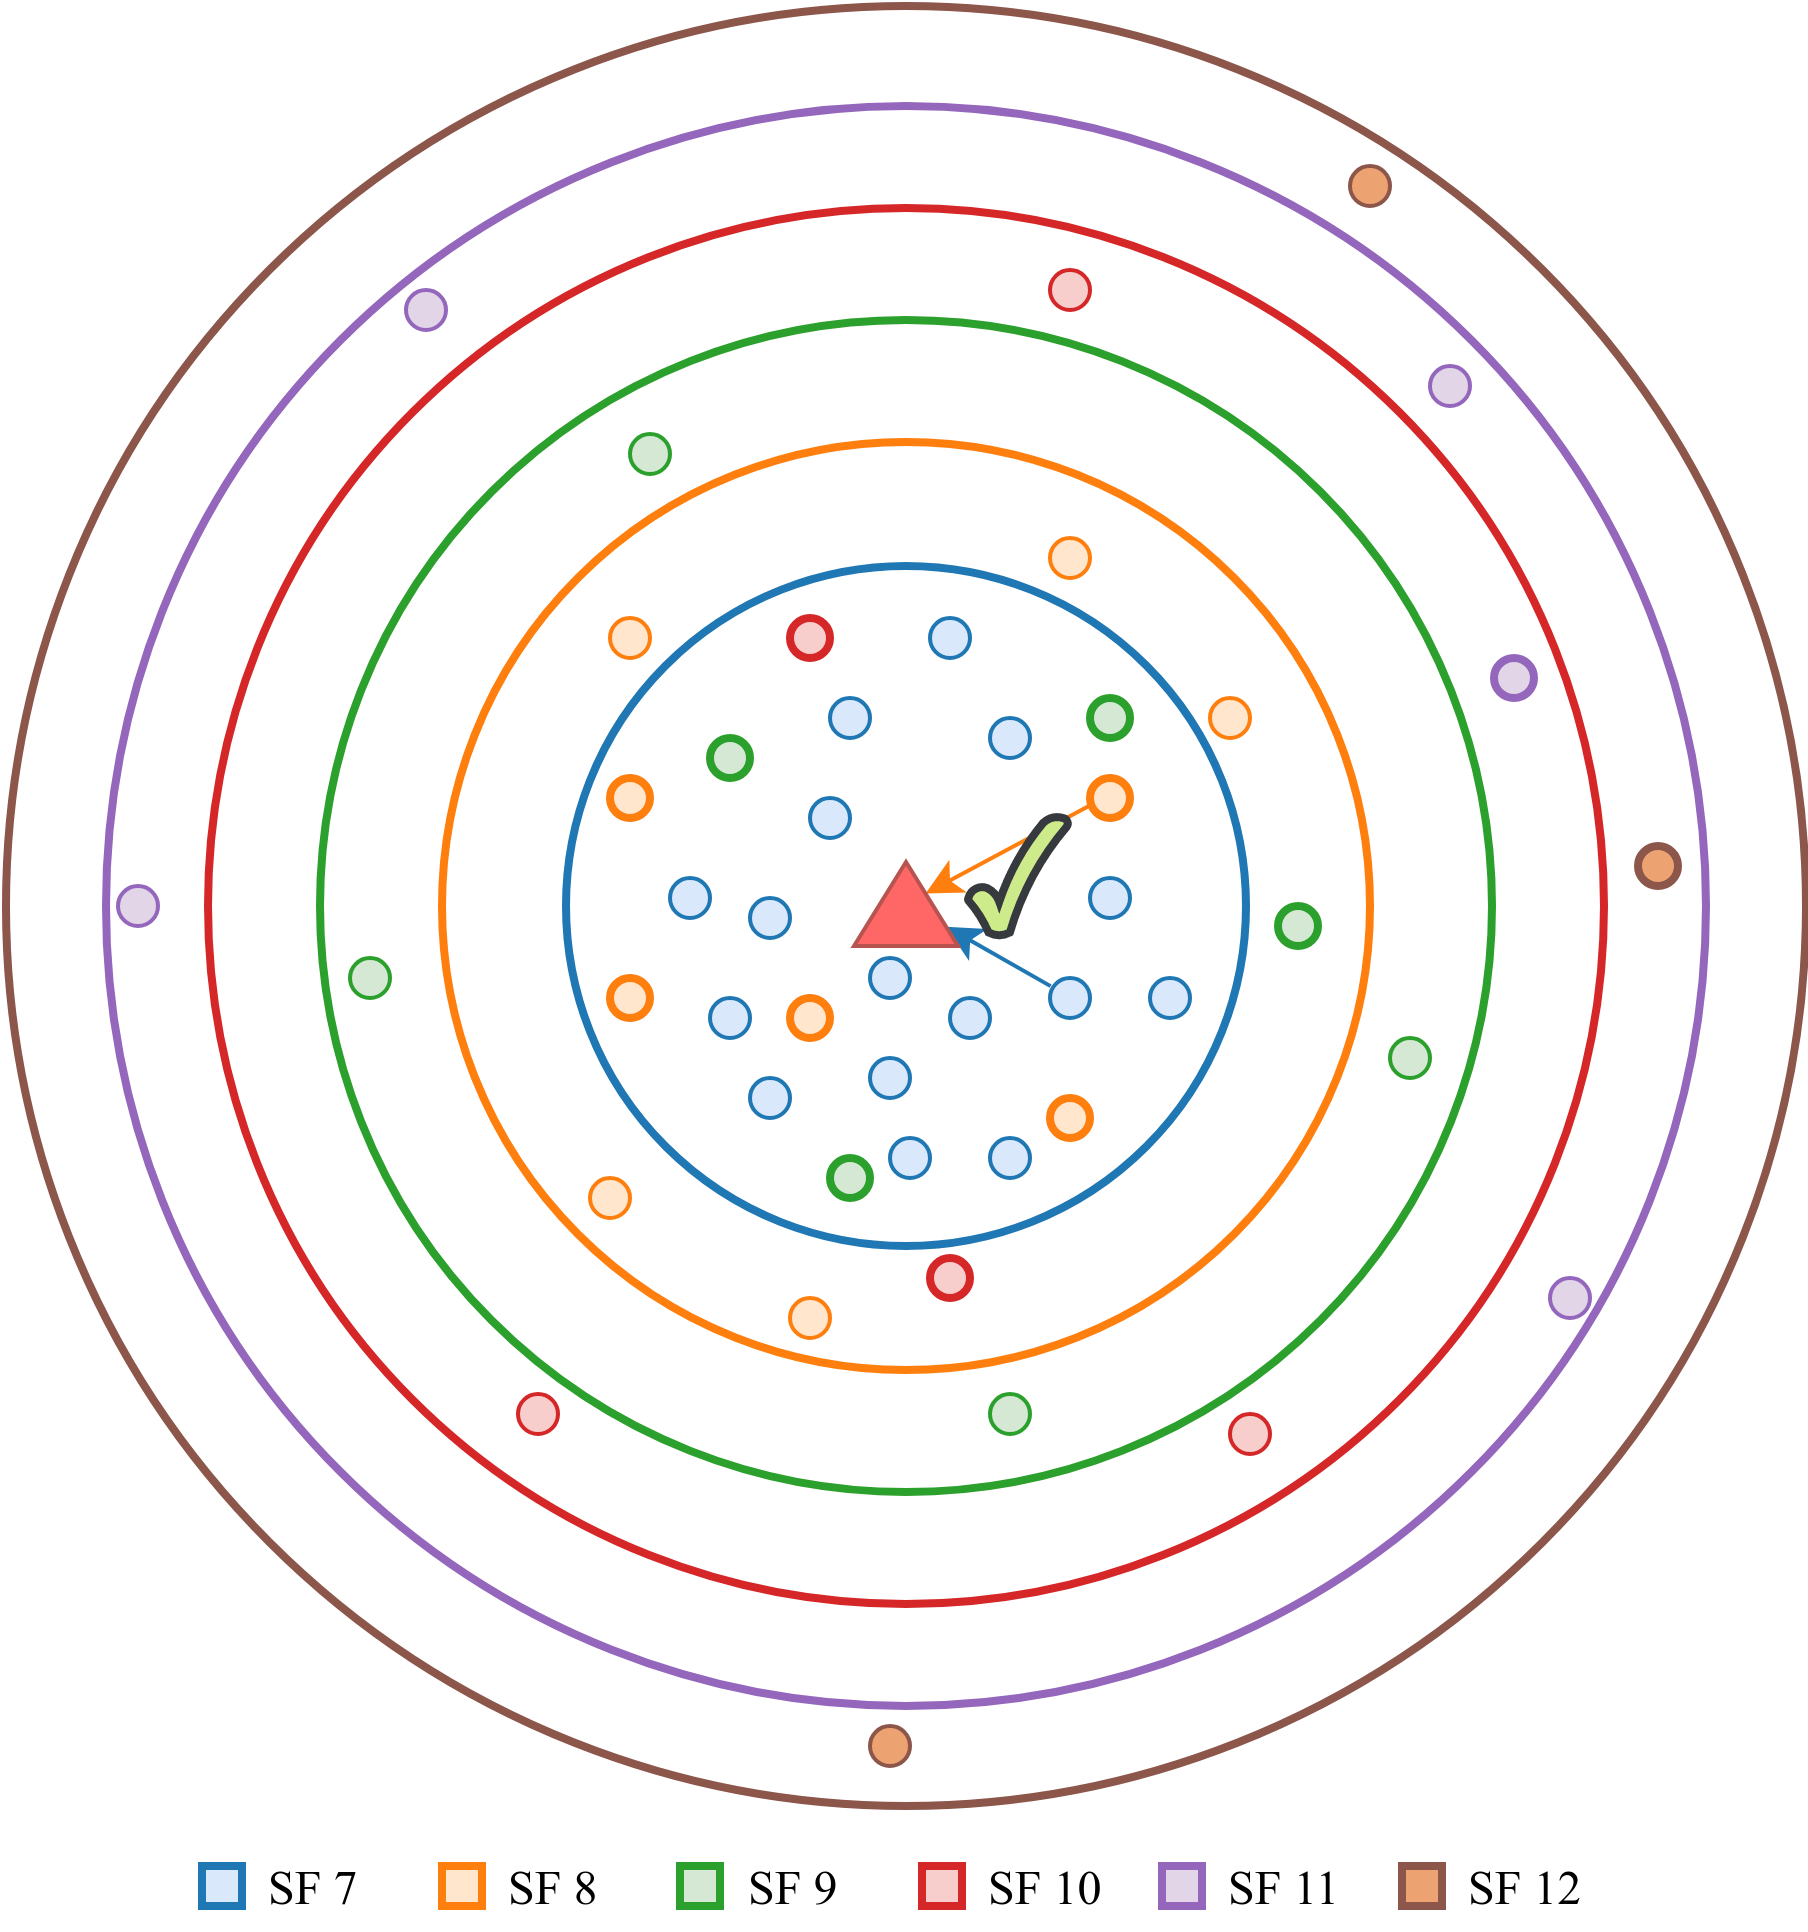
\includegraphics[width=\linewidth]{collision_solution_single_gw}
\caption{Collision avoidance by using higher SF for nodes close to the GW.}
\label{fig:collision_solution_single_gw}
\end{figure}

\begin{figure}
\centering
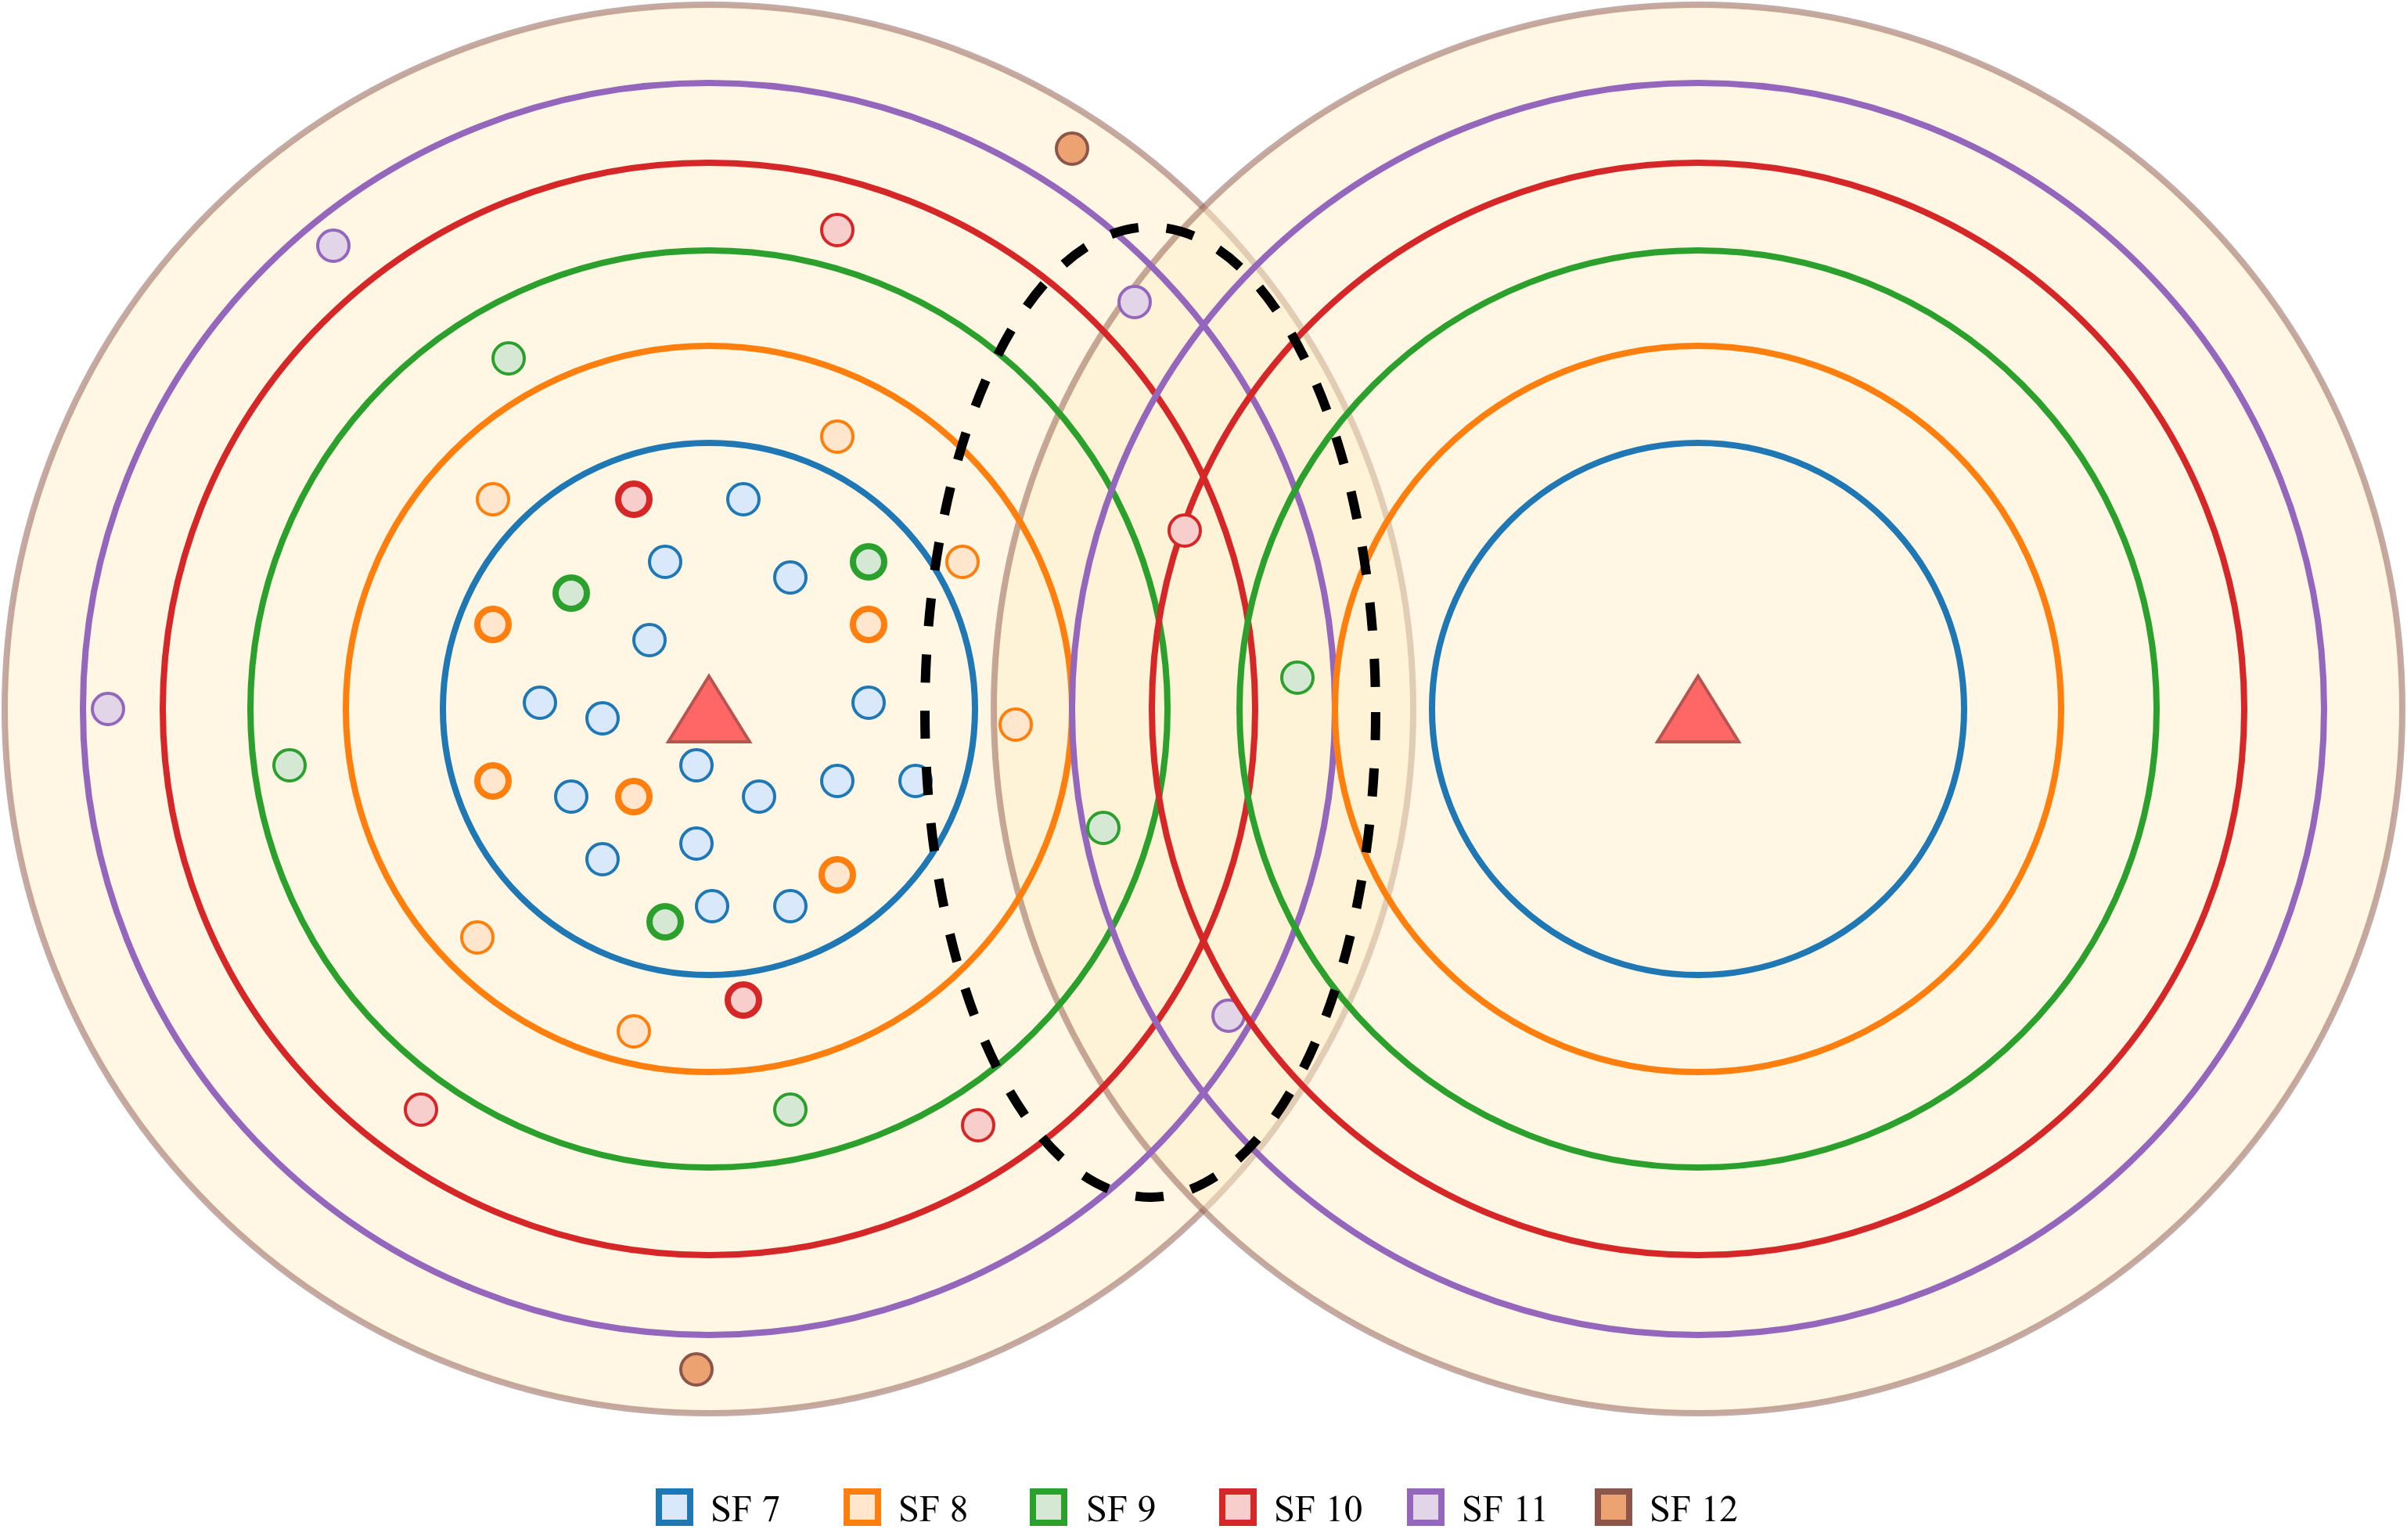
\includegraphics[width=\linewidth]{collision_solution_multi_gw}
\caption{Collision avoidance for intersecting GWs.}
\label{fig:collision_solution_multi_gw}
\end{figure}


\section{Simulation Environment} \label{Simulation Environment}
\par A discrete event simulator is implemented in Python to study effects of different SF strategies in LoRaWANs. The LoRaWAN SF simulation tool source code is available at \cite{simlorasf}. Simulation tool supports custom LoRaWAN topologies as well as randomly generated LoRaWAN topologies. Simulator can generate uniformly distributed circular shape network topology with radius (m), number of nodes and number of gateways input parameters. Global simulation input parameters are simulation duration (s), packet size (B), packet generation rate (p/s) and spreading factor assignment method. With these inputs, the simulator provides outputs of total number of generated packets, number of successfully received packets, number of interfered packets, number of under sensitivity packets, network packet delivery ratio percentage (PDR), network throughput (bps) and total transmit energy consumption (J).

\par In the simulator, only LoRaWAN Class A devices are covered. Transmissions are always initiated by end nodes in pure ALOHA manner. Nodes generate a new packet according to Poisson interval for given packet rate input parameter. In the simulator, downlink transmissions are not considered. Downlink transmissions are rare in real world deployments since ISM band regulations dictates duty cycle limit for all devices including GWs.

\subsection{Link Model}
\par Link quality of a wireless system can be expressed by the metric of link budget. Link budget is a measure of all gains and losses from transmitter device to receiver device. Link budget of a wireless link can be calculated as \cite{AN1200.22}:

\begin{equation} \label{eq:expected_rx_power}
P^{dBm}_{RX} = P^{dBm}_{TX} + G^{dB}_{SYS} - L^{dB}_{SYS} - L^{dB}_{PATH}
\end{equation}

\par Where, $P^{dBm}_{RX}$ is the expected receive power at the receiver. $P^{dBm}_{TX}$ is the transmit power of the transmitter. $G^{dB}_{SYS}$ is the system gains such as transmitter and receiver antenna gains. $L^{dB}_{SYS}$ is the system losses such as transmitter and receiver line, circuit, antenna losses. $L^{dB}_{PATH}$ is the propagation path loss between transmitter and receiver antennas in open space. In the simulator, it is assumed that total of system gains $G^{dB}_{SYS}$ and system losses $L^{dB}_{SYS}$ is +7 dB.

\par In the simulator, it is assumed that nodes always select maximum allowed transmit power, which is 14 dBm for European ISM band regulation. Different channel transmissions are independent from each other. But, in this work we focus on SF orthogonality. Thus, we only utilized single channel transmissions in the simulator.

\par Receive sensitivity of a LoRa gateway for different SFs and BWs in dBm unit can be found in \cite{SX1276}. In the simulator, 125 kHz bandwidth receive sensitivities are used.

\par Free space propagation loss is calculated as in \cite{TR136.942}. In this work, it is assumed that $h$ = 15 m and $f$ = 868 MHz.

\par If the received signal power is higher than the gateway sensitivity, then signal can be decoded by the receiver successfully when there is no interfering transmission at the duration of transmission.

\subsection{Interference Model}
\par In the simulator, interference model described in \cite{7996384} is adopted. They use SINR threshold matrix for modeling LoRa interference between simultaneous but different SF LoRa transmissions.

\par In our simulator, it is assumed that there is no other technology interference in the network except LoRa interference. To exploit imperfect orthogonality of different SF transmission, simulator should calculate the effect of different SF transmissions to each other. In simulator, following signal to interference plus noise ratio (SINR) threshold matrix from \cite{goursaud:hal-01231221} is used.

\par To decide if a referenced signal is interfered at receiver by a interferer signal, SINR threshold matrix is used. $T_{i,j}$ is the needed SINR margin in dB unit between referenced signal with SF = i and interferer signal with SF = j to correctly decode the referenced signal. If there are more than one interferer, referenced signal must satisfy the margin for cumulative sum of all interfering signal received powers for each SF \cite{7996384}. Transmission duration of a packet can be calculated by data rate $R_{b}$ and packet size $PS$. Data rate of a LoRa transmission is already expressed in Equation \ref{eq:bit_rate_sf}.

\section{Simulation Results}  \label{Simulation Results}
\par For simulation results in this paper, global simulation parameters are set as follows. Packet size is 60 bytes including header and payload, simulation duration is 3600 seconds, packet generation rate is 0.01 packet per second.

\par In Figure \ref{fig:sf_pdr}, PDR plot of different SF assignment is shown. Randomly generated network topology radius is set to 3000 meters and number of GW is set to 1. Increasing SFs increases time on air. This increases the number of collisions thus decreases the PDR of the network. PDR of higher SFs are decreased to almost 0 while number of nodes is increasing. Since network topology radius is quite small almost all SFs can reach to the GW.

\begin{figure}
\centering
\includegraphics[width=\linewidth]{{sf_pdr_r3000_g1_p0.01_s3600}.png}
\caption{PDR of different SFs.}
\label{fig:sf_pdr}
\end{figure}

\par In Figure \ref{fig:gw_pdr}, PDR plot of different number of GW is shown. Randomly generated topology radius is set to 3000 meters and lowest possible SF assignment scheme is used. Increasing number of GWs, decreases the SFs of nodes and decreases time on air. This decreases number of collisions thus increases the PDR of the network when network topology radius is constant.

\begin{figure}
\centering
\includegraphics[width=\linewidth]{{gw_pdr_r3000_p0.01_s3600}.png}
\caption{PDR of different number of gateways.}
\label{fig:gw_pdr}
\end{figure}

\par In Figure \ref{fig:r_pdr}, PDR plot of different network topology radius is shown. Number of GW is set to 1 and lowest possible SF assignment scheme is used. Increasing network topology radius, increases the number of under sensitivity transmissions thus decreases the PDR of the network.

\begin{figure}
\centering
\includegraphics[width=\linewidth]{{r_pdr_g1_p0.01_s3600}.png}
\caption{PDR of different topology radius.}
\label{fig:r_pdr}
\end{figure}

\par For space constraints, we omit figures for network throughput output, total transmit energy consumption output and different packet generation rate input. We invite readers to experiment the simulation tool with different simulation inputs and outputs. \cite{simlorasf}.

\par In Figure \ref{fig:prediction_pdr}, PDR plot of machine learning prediction scheme is shown. Randomly generated network topology radius is set to 5000 meters and number of GW is set to 3. Prediction model needs nodes location so three GWs are used for prediction SF scheme since three GWs are enough to roughly locate nodes positions by triangulation. Prediction scheme gives better PDR when number of nodes increases since number of interferences also increases. Prediction scheme can only improve network performance when LoRa interference is present. Also, prediction scheme gives better results when nodes are deployed close to the gateway, since nodes have margin to increase their SFs. If a node is far away from the GW, then prediction scheme cannot increase the SF to avoid interference since the SF is already high.

\begin{figure}
\centering
\includegraphics[width=\linewidth]{{prediction_pdr_r5000_g3_p0.01_s3600}.png}
\caption{PDR of SF prediction scheme.}
\label{fig:prediction_pdr}
\end{figure}

\par In Table \ref{table:prediction_pdr}, TODO

\par In Table \ref{table:prediction_accuracy}, TODO

\begin{table}
\centering
\caption{PDR of lowest possible SF and smart SF assignment schemes.}
\label{table:prediction_pdr}
\begin{tabular}{|c|c|c|c|c|c|}
\hline
\multicolumn{3}{|c|}{\multirow{2}{*}{}}                            & \multicolumn{3}{c|}{\textbf{Number of Nodes}} \\ \cline{4-6}
\multicolumn{3}{|c|}{}                                             & 100           & 500           & 1000          \\ \hline
\multirow{12}{*}{\textbf{R (m)}} & \multirow{3}{*}{3000}  & Lowest & 97.8          & 86.0          & 72.3          \\ \cline{3-6}
                                 &                        & SVM    & 98.0          & 88.2          & 75.2          \\ \cline{3-6}
                                 &                        & DTC    & 97.8          & 89.8          & 78.7          \\ \cline{2-6}

                                 & \multirow{3}{*}{5000}  & Lowest & 96.8          & 85.5          & 71.2          \\ \cline{3-6}
                                 &                        & SVM    & 98.0          & 87.8          & 74.8          \\ \cline{3-6}
                                 &                        & DTC    & 97.7          & 90.2          & 79.8          \\ \cline{2-6}

                                 & \multirow{3}{*}{7000}  & Lowest & 97.2          & 87.5          & 76.8          \\ \cline{3-6}
                                 &                        & SVM    & 98.2          & 88.8          & 78.6          \\ \cline{3-6}
                                 &                        & DTC    & 97.8          & 90.7          & 81.6          \\ \cline{2-6}

                                 & \multirow{3}{*}{10000} & Lowest & 98.2          & 90.3          & 81.5          \\ \cline{3-6}
                                 &                        & SVM    & 98.3          & 90.3          & 81.9          \\ \cline{3-6}
                                 &                        & DTC    & 98.3          & 90.6          & 81.9          \\ \hline
\end{tabular}
\end{table}

\begin{table}
\centering
\caption{Prediction accuracy (\%) of SVM and DTC classifiers.}
\label{table:prediction_accuracy}
\begin{tabular}{|c|c|c|c|c|c|}
\hline
\multicolumn{3}{|c|}{\multirow{2}{*}{}}                        & \multicolumn{3}{c|}{\textbf{Number of Nodes}} \\ \cline{4-6}
\multicolumn{3}{|c|}{}                                         & 100           & 500           & 1000          \\ \hline
\multirow{8}{*}{\textbf{R (m)}} & \multirow{2}{*}{3000}  & SVM & 82.4          & 70.4          & 71.7          \\ \cline{3-6}
                                &                        & DTC & 86.0          & 67.3          & 70.4          \\ \cline{2-6}

                                & \multirow{2}{*}{5000}  & SVM & 79.5          & 69.0          & 71.1          \\ \cline{3-6}
                                &                        & DTC & 84.5          & 67.3          & 69.5          \\ \cline{2-6}

                                & \multirow{2}{*}{7000}  & SVM & 79.5          & 70.6          & 71.2          \\ \cline{3-6}
                                &                        & DTC & 84.5          & 67.7          & 69.2          \\ \cline{2-6}

                                & \multirow{2}{*}{10000} & SVM & 79.2          & 74.4          & 76.1          \\ \cline{3-6}
                                &                        & DTC & 83.8          & 70.7          & 74.3          \\ \hline
\end{tabular}
\end{table}

\section{Conclusion} \label{Conclusion}
\par In this paper, after a brief introduction about LPWAN technologies, we provide background information about one of the most promising LPWAN technology, LoRa. Then, we discuss about LoRa modulation basics and spreading factor assignment issue. We have implemented a discrete event simulator from scratch to study network performance of LoRaWAN and evaluate different SF assignment schemes. We have shown how same SF transmission collisions can be avoided and we proposed a machine learning based solution for collision with same SF transmissions. We illustrate simulation results for proposed machine learning SF assignment technique. Our simulation results show that, proposed technique can increase network performance for LoRaWAN networks when nodes are deployed close to the GWs.

\par As for future works, transmit power optimization can be included to proposed machine learning scheme. In this paper, we assume that nodes always use maximum transmit power for uplink transmission, however nodes close to the GW can decrease transmit power to save energy. This will make transmissions to more vulnerable to interference thus requires extra care. Also, other machine learning methods can be investigated for SF optimization. Reinforcement learning is a good candidate for this network optimization issue. Other transmission parameters such as node id and transmission time can be included to proposed scheme to improve performance.


\section*{Acknowledgment}
\par This work is supported by Turkish Ministry of Development and Istanbul Technical University researcher support program under the Grant No. ITU-AYP-2017-1.


\bibliographystyle{IEEEtran}
\bibliography{references}

\end{document}
